% SPDX-FileCopyrightText: 2024 Lukas Zirpel <thesis+lukas@zirpel.de>
% SPDX-License-Identifier: GPL-3.0-only

\chapter{Methodology}
\label{chap:methodology}

\section{Experimental design}
\begin{itemize}
	\item Was haben wir vor?
	\item Wie können wir das erreichen?
	\item Was müssen wir dabei beachten?
\end{itemize}
We want to measure the overhead of encryption and censorship evasion protocols over lossy links.
Therefore we need a measurement setup, which allows us to do so.
It should offer repeatability and consistency.
It should include a traffic generator which generates the simplest possible traffic pattern, a constant stream of data.
The stream of data should only flow in one direction and should not attempt to do congestion control as we don't want to evaluate congestion control algorithms but 
The setup should allow simulating different network conditions.
The data traffic should flow from the traffic generator, be encoded differently by the censorship protocol, pass through the network emulator and finally be decoded by the censorship protocol.
capture all packets in their original form so we can tweak the analysis later without rerunning all tests again
analyze packet captures later (post-experiment analysis)
need to be careful with synchronization of timestamps between different points
It should also be easy to add new protocols and experiment with the setup both for us and for future researchers wishing to tweak the setup or test more protocols.

\section{Testbed}
\begin{itemize}
  \item Was haben wir zusammengesteckt (Figure)
  \item Warum Hardware und nicht virtuell?
  \item Warum Nix?
\end{itemize}
\begin{figure}[tbh]
	\centering
	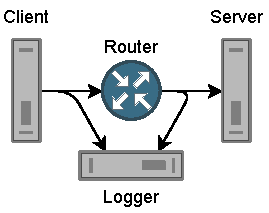
\includegraphics[draft=false,width=0.4\textwidth]{figures/Network schematic/actual/setup.pdf}
	\caption{Our Network Setup}\label{fig:actual_network_schematic}
\end{figure}
\begin{figure}[tbh]
	\centering
	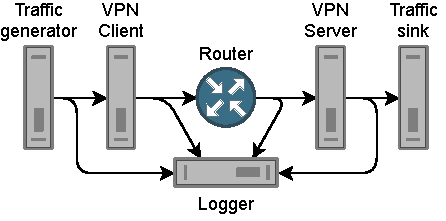
\includegraphics[draft=false,width=0.7\textwidth]{figures/Network schematic/optimal/setup.pdf}
	\caption{Improved Network Setup}\label{fig:optimal_network_schematic}
\end{figure}
There are a number of \textit{existing network simulators} \cite{network-simulators-list} for simulating complex network setups with routers, switches, etc..
Many of them focus on simulating mesh networks for testing routing protocols, for example \textit{Mesh Network Lab} \cite{meshnet-lab}.
Our network is relatively simple, while the complexity lies in the configuration of the hosts.
This is part of the reason why we chose the NixOS testing framework for our first prototypes.
It allows declararing the exact configuration of the hosts and the virtual network in code.
All dependencies are pinned in a lock file and no outside dependencies are used so everything should still be reproducible in a decade or more without having to distribute gigabytes of VM or container images while still being able to easily modify any part of the system.

First we use the NixOS testing framework for prototyping and then transfer the setup to bare-metal hardware.
The NixOS testing framework launches several VMs with QEMU and sets up a virtual network switch.
Using the NixOS testing framework we declare the configuration of all four hosts as well as the network topology in Nix code.
We also specify a test script, which imperatively executes one command at a time.
We roughly execute these steps: start all hosts, wait for them to be ready, tell the router to emulate the network conditions we want, start the traffic generator, wait for it to be done and finally collect the packet captures.
We store the packet captures for later analysis.


For real measurements we installed NixOS on PCs, which are centrally controlled from a custom measurement harness.
It is designed to be compatible enough with the NixOS testing framework to work with the same test script.



Nix is not really designed for this use-case as it isolates the build steps in a sandbox with no network access and 
we disable the sandbox, allowing SSH to reach all the machines
this invalidates some guarantees Nix normally provides.
does not ensure an SSH key was generated, that the four machines are running or that OS running on the machines is what was expected
nevertheless
if Nix got in the way after running the measurements, can also be easily copied out of the Nix store by specifying the measurements you want to export in \todo{file path here} and running \todo{nix build .\#measurements}

store results in Nix store for easy processing by the pipeline
downside: have to be careful to not modify the test script, otherwise tests will be run again, could also be seen as a positive to prevent modifications that "should" not influence the results but actually do.
positive side: when modifying any part of the pipeline, only the modified and later parts will be rerun, no need to manually run only the appropriate parts of the pipeline, which is tedious and error-prone or rerun the entire pipeline every time, which is time consuming.


In the VM test setup, the virtual switch is configured to behave like a \textit{hub} \cite{wiki:Ethernet_hub} \cite{NixOS-VM-test-Hub}, which makes it easy to capture the packets on both VLANs.
On real hardware with a real switch, this is not quite as trivial.
To replicate this setup with real hardware, we use Cisco's Switched Port Analyzer (SPAN), also known as port mirroring.
Since enabling SPAN disables our ability to transmit packets from that interface for management purposes, we use a USB to Ethernet adapter for the management interface.
Switch has 100MBit/s and 1GBit/s ports
three PCs connected to 100MBit/s, limiting bandwidth therefore 100MBit/s, thanks to full duplex on the link between router and switch
monitor port of logger connected to 1GBit/s port to keep up with 200MBit/s maximum data rate
iperf send with 100MBit/s
Switch has 100MBit/s and 1GBit/s ports
three PCs connected to 100MBit/s, limiting bandwidth therefore 100MBit/s, thanks to full duplex on the link between router and switch
monitor port of logger connected to 1GBit/s port to keep up with 200MBit/s maximum data rate
iperf send with 100MBit/s
first vm setup for experimentation
then real hardware to eliminate variables
while it is possible to build a reliable benchmarking setup using virtual machines, ...
one less variable

\subsection{Hardware used}
\begin{table}[]
	\centering
	\footnotesize
	\begin{tabular}{cl}
		\toprule
		\textbf{Category} & \textbf{Details}                                                                                       \\ \midrule
		\rowcolor[HTML]{EFEFEF}
		Switch            & Catalyst 6500 Series Switch (TBD)                                                                      \\ \midrule
		PCs               & DELL OptiPlex 7070 Micro                                                                               \\
		\rowcolor[HTML]{EFEFEF}
		& INTEL® CORE™ i5-9600 (6 cores, 3.1GHz)                                                                 \\
		& \begin{tabular}[c]{@{}l@{}}16GB RAM\\ One 2666 MHz DDR4 SODIMM module,\\ HMA82GS6JJR8N-VK\end{tabular} \\
		\rowcolor[HTML]{EFEFEF}
		& 512GB NVME SSD                                                                                         \\ \midrule
		SBCs              & Orange Pi Zero3                                                                                        \\
		\rowcolor[HTML]{EFEFEF}
		& Allwinner H618 Cortex-A53 (4 cores, 1.5GHz)                                                            \\
		& 2GB RAM                                                                                                \\
		\rowcolor[HTML]{EFEFEF}
		& 32GB microSD card                                                                                      \\ \bottomrule
	\end{tabular}
	\caption{Hardware used}
	\label{tab:hardware}
\end{table}

\section{Scenario Selection}
\subsection{Protocols to test}
\begin{itemize}
  \item none, as a baseline
  \item WireGuard
  \item DNS tunnel (iodine)
  \item ICMP tunnel (ICMPTX)
  \item phantun
  \item Various Tor Protocols
\end{itemize}

\todo{provide reasoning why we chose these protocols specifically and describe them briefly}

\subsection{Parameters to test}
\begin{table}[]
	\centering
	\footnotesize
	\begin{tabular}{cccccc}
		\toprule
		\textbf{Parameter} & \textbf{Loss} & \textbf{Delay} & \textbf{Jitter} & \textbf{Duplicate} & \textbf{MTU} \\ \midrule
		\rowcolor[HTML]{EFEFEF}
		Unit               & \%            & ms             & ms              & \%                 & Bytes        \\
		& 0             & 0              & 0               & 0                  & 1400         \\
		\rowcolor[HTML]{EFEFEF}
		& 0.1           & 1              & 10              & 2                  &              \\
		& 0.2           & 10             &                 & 100                &              \\
		\rowcolor[HTML]{EFEFEF}
		& 0.5           & 50             &                 &                    &              \\
		& 1             & 100            &                 &                    &              \\
		\rowcolor[HTML]{EFEFEF}
		& 10            & 200            &                 &                    &              \\
		& 50            & 1000           &                 &                    &              \\
		\rowcolor[HTML]{EFEFEF}
		& 100           &                &                 &                    &              \\ \bottomrule
	\end{tabular}
	\caption{Sampling the Parameters}
	\label{tab:parameters}
\end{table}
explain why these parameters







In an attempt to save space...
The \textit{.pcap} \cite{wiki:Pcap} files only compress well if the data is not encrypted or otherwise scrambled.
The files could either be explicitly compressed with a compression tool like zstd or the compression could be done at the filesystem level, e.g. with \textit{OpenZFS} \cite{OpenZFS}. \todo{Btrfs}


Since we're only interested in measuring what happens during the actual test and not in the connection setup and teardown of iperf3, we use heuristics
The connection setup and teardown of iperf3 should not be part of the analysis, hence a heuristic is employed to ignore this part of the packet capture.
To find the start of the test, we find the first packet which is larger than a threshhold.
To find the end of the test, we find the last packet which is larger than a threshhold and also ignore all packets that are sent after the duration of the test is over.

\todo{go through presentation and extract the info here}

\textit{nixos-anywhere} \cite{nixos-anywhere} is used to quickly and reproducibly install the operating system on all machines.
nixos-anywhere uses \textit{disko} \cite{disko} to partition and format the disks.


\todo{Define pre and post to mean before and after the router}

Data analysis pipeline:
\begin{itemize}
  \item run the measurement setup
  \item capture packets before and after the router and store them in .pcap files
  \item for each packet, extract the timestamp and compute the size and \textit{BLAKE3} \cite{wiki:BLAKE3} hash of the IP payload and write the information into a \textit{JSON} \cite{wiki:JSON} file (done in analysis/parse/parse.py)
  \item for each packet captured before the router, find the same packet after the router (done in analysis/statistics/statistics.py). If we assume, that all packets are unique and that the router does not modify packets, then we can match up the unique hash of each packet before the router to some number of packets after the router. If no matching packet can be found after flowing through the router, it means that the packet was dropped. If more than one packet matches, it means that it was duplicated. If exactly one packet matches, it was routed without duplication or being dropped. For meaningful statistics, we group the data into short chunks (buckets) (1s) and compute bandwidth and packet counts over that bucket. The latency introduced by the router can be measured by computing the difference between the timestamps of each packet before the router and the first corresponding packet after the router. Dropped packets are ignored and for duplicated packets only the first arriving packet is counted. Throughput can be measured by summing up the IP payload \todo{should we measure at a different layer?} and dividing it by the time duration of the bucket. Dropped packets are ignored and packets which were duplicated count only once. The timestamp, dropped, duplicated and normal packet counts, throughput and a list of the latency of each packet are stored per bucket and written to a JSON file.
  \item Graphs are drawn using \textit{Matplotlib} \cite{Matplotlib} (done in analysis/graph/graph.py)
  \item \todo{for gaining insights, for example while comparing two different scenarios, it's helpful to plot data from multiple measurements in one plot. This still needs to be implemented.}
\end{itemize}


\todo{explain why we're capturing packets on a separate host.}
We're capturing packets on a separate host to make sure the measurement does not influence the rest of the test setup, e.g. through higher CPU utilization of a host.
\todo{also talk about avoiding the need for clock synchronization}


Because Nix has the properties mentioned in \ref{Nix-explanation}, we use it in our methodology.


For reproducing the software exactly, we use Nix and NixOS.
All systems, testing scripts and the data analysys pipeline can be reproduced almost perfectly this way with very little effort.



\cite{RFC7858}
